\documentclass{article}

\usepackage{../preamble}
\standalonetrue

\pagestyle{fancy}
\fancyhf{}
\rhead{Section \thesection}
\lhead{PHYS 304 Lecture 16}
\rfoot{Page \thepage}


\title{PHYS 304 Lecture 16}
\author{Ashtan Mistal}
\date{!!!}

\begin{document}

\ifstandalone
\maketitle
\fi

\graphicspath{{./Lecture16/}}



%[slide 2]

\section{Review of key points from last lecture}

Saw several more examples of how to transform equations in Dirac notation into equations involving wavefunctions and differential/integral operators in any viable basis. Ended up deriving a series of basis transformation equations that could be used to convert the wavefunction of some state in one basis, into the wavefunction of the same state expressed in a different basis.

We generalized the notion of our old friend, $|\Psi(x,t)|^2$ as a probability density of finding the particle at some location $x$, to take account of the fct that wavefunctions of a fixed stats $\ket{S(t)}$, can have many different wavefunction representations in different bases. 

\textbf{WE interpret, for good reason, $|Psi_{\ket{S(t)}}(M_n,t)|^2$ as the probability distribution function of finding the particle with some eigen value $M_n$ of the observable operator $\hat{M}$, when that particle is in the state $\ket{S(t)}$ that is a solution of the Schrodinger equation. Explicitly, $\Psi_{\ket{S(t)}}(M_n,t) = \braket{M_n|S(t)}$, where $\ket{M_n}$ is an eigen state of the observable operator $\hat{M}$; $\hat{M} \ket{M_n} = M_n \ket{M_n}$ with eigen value $M_n$. }


\section{Today: Generalized Statistical Interpretation}

\begin{itemize}
    \item Elaborate slightly on the last point from Lecture 15
    \item Derive the “Generalized Uncertainty Relationship” between the variances of any two physical observables.
    \item Discuss some implications of this uncertainty principle.
\end{itemize}
\begin{quote}
    \textbf{WE interpret, for good reason, $|Psi_{\ket{S(t)}}(M_n,t)|^2$ as the probability distribution function of finding the particle with some eigen value $M_n$ of the observable operator $\hat{M}$, when that particle is in the state $\ket{S(t)}$ that is a solution of the Schrodinger equation. Explicitly, $\Psi_{\ket{S(t)}}(M_n,t) = \braket{M_n|S(t)}$, where $\ket{M_n}$ is an eigen state of the observable operator $\hat{M}$; $\hat{M} \ket{M_n} = M_n \ket{M_n}$ with eigen value $M_n$. }
\end{quote}

This can be further interpreted as meaning that if you carry out a measurement of any observable with the particle in some state $\ket{S(t)}$ at time $t$, with sufficient resolution, you must measure one of the eigen values of that observable, and the state will be collapsed immediately after the measurement to the corresponding eigen state.  (This is obviously most straight-forwardly interpreted if the eigen spectrum is discrete.)  The probability of measuring any one eigen value is given by the squared magnitude of the wavefunction of $\ket{S(t)}$ in the basis of the observable being measured.

What would be one way of preparing a state with zero variable in some observable?

\begin{itemize}
    \item Make a measurement of that particle [with infinite precision]. Once we measure it, we force it to be at that value with the eigen state. 
\end{itemize}

$$\braket{M|\left( \hat{M} - \bar{M} \right)^2|M} = \braket{M| \hat{M}^2 - \bar{M}^2 | M} = 0 \text{ in an eigen state}$$

$\braket{M|\left( \hat{M} -\bar{M} \right)^2|M} \propto $ variance of $M$

If some other observable shared the same set of eigenstates, what would be the variance of that other observable after the state is prepared as above? \textit{(zero)}

If two operators $\hat{A}$ and $\hat{B}$ have the property that $\hat{A} \hat{B} = \hat{B} \hat{A}$, then they must share a common set of eigen states. 

If $\hat{A} \hat{B} - \hat{B} \hat{A} = 0$, then they share a common set of eigen states. 

$\hat{A} \ket{A} = A \hat{A}$, and $\therefore \hat{B} \hat{A} \ket{A} = A \hat{B} \ket{A}$. 

This is also equal to $\hat{A} \left( \hat{B} \ket{A} \right) = A \left( \hat{B} \ket{A} \right)$. then $\Longrightarrow \hat{B} \ket{A}$ is also an eigen state of $\hat{A}$, with eigen value $A$ $\Longrightarrow \hat{B} \ket{A} = c \ket{A}$ where $c$ = some value.

Does this tell us what the eigen value of the observable B is in this eigen state of A?

This does not tell us anything about what the eigen \textbf{values} of the operators. 

What does this imply for the precision with which one could measure the observables corresponding to two commuting operators when the particle is in one of their shared eigen states?  

\subsection{The Generalized Uncertainty Relation}

We have previously in the course made observations about the apparent relationship between the “degree of localization” of a quantum particle in position space, a measure of which is the variance of the position operator in a particular state, and the “degree of localization” of the same state in momentum space, a measure of which is the variance of the wavefunction’s Fourier transform.  POLL: WHAT IS THIS RELATIONSHIP? A) proportional B) inverse C) Equal

% answer is b

In particular, as intuitively reinforced using the Fourier Series simulation tool, there seems to be an inverse relationship between the variances of the state in position space and in momentum or wavevector space (i.e. the more localized in position (momentum) space, the less localized will be the state in momentum (position) space).  We are now going to prove the following, more general relationship between the variances of any two physical observables, $A,B$, represented by Hilbert space operators $\hat{A}, \hat{B}$?

$$\sigma_A^2 \sigma_B^2 \geq \left( \frac{1}{2i} \langle \left[ \hat{A}, \hat{B} \right] \rangle \right)^2$$

$$\sigma_A^2 = \braket{S|(\hat{A} - \bar{A})^2|S} = \braket{S|(\hat{A} - \bar{A} )(\hat{A} - \bar{A})|S} = \langle (\Delta \hat{A} \ket{S}) | \Delta \hat{A} \ket{S})$$

where $\hat{A} =\ket{S|\hat{A}|S}$, and $\Delta \hat{A} = \left(\hat{A} - \bar{A} \right)$. Here we needed to use the fact that $\hat{A}$ is Hermitian. 

Similarly for an observable B,

$$\sigma_B^2 = \braket{S|(\hat{B} - \bar{B})^2|S} = \braket{S|(\hat{B} - \bar{B} )(\hat{B} - \bar{B})|S} = \langle (\Delta \hat{B} \ket{S}) | \Delta \hat{B} \ket{S})$$

%[insert slide 9]
%,missing vertical bar on line 3 of actual math; missing vertical bar in the middle between two round brakets and closing ket. 

$$\sigma_A^2 \sigma_B^2 = \braket{\Delta AS|\Delta AS} \braket{\Delta BS| \Delta BS}$$

From the Schwartz inequality of linear algebra, 

$$\bra{\left( \Delta \hat{A} \ket{S} \right)} \left( \Delta \hat{A} \ket{S} \right) \bra{(\Delta \hat{B} \ket{S})} \left( \Delta \hat{B} \ket{S} \right) \geq \left| \langle \left( \Delta \hat{A} \ket{S} \right) | \left( \Delta \hat{B} \ket{S} \rangle \right)  \right|^2$$

Now $\left| \langle \left( \Delta \hat{A} \ket{S} \right) | \left( \Delta \hat{B} \ket{S} \rangle \right)  \right|^2$ is some complex number, and the squared magnitude of any complex number is always greater than the squared magnitude of its imaginary part, and hence:

[insert rest of slide 9]

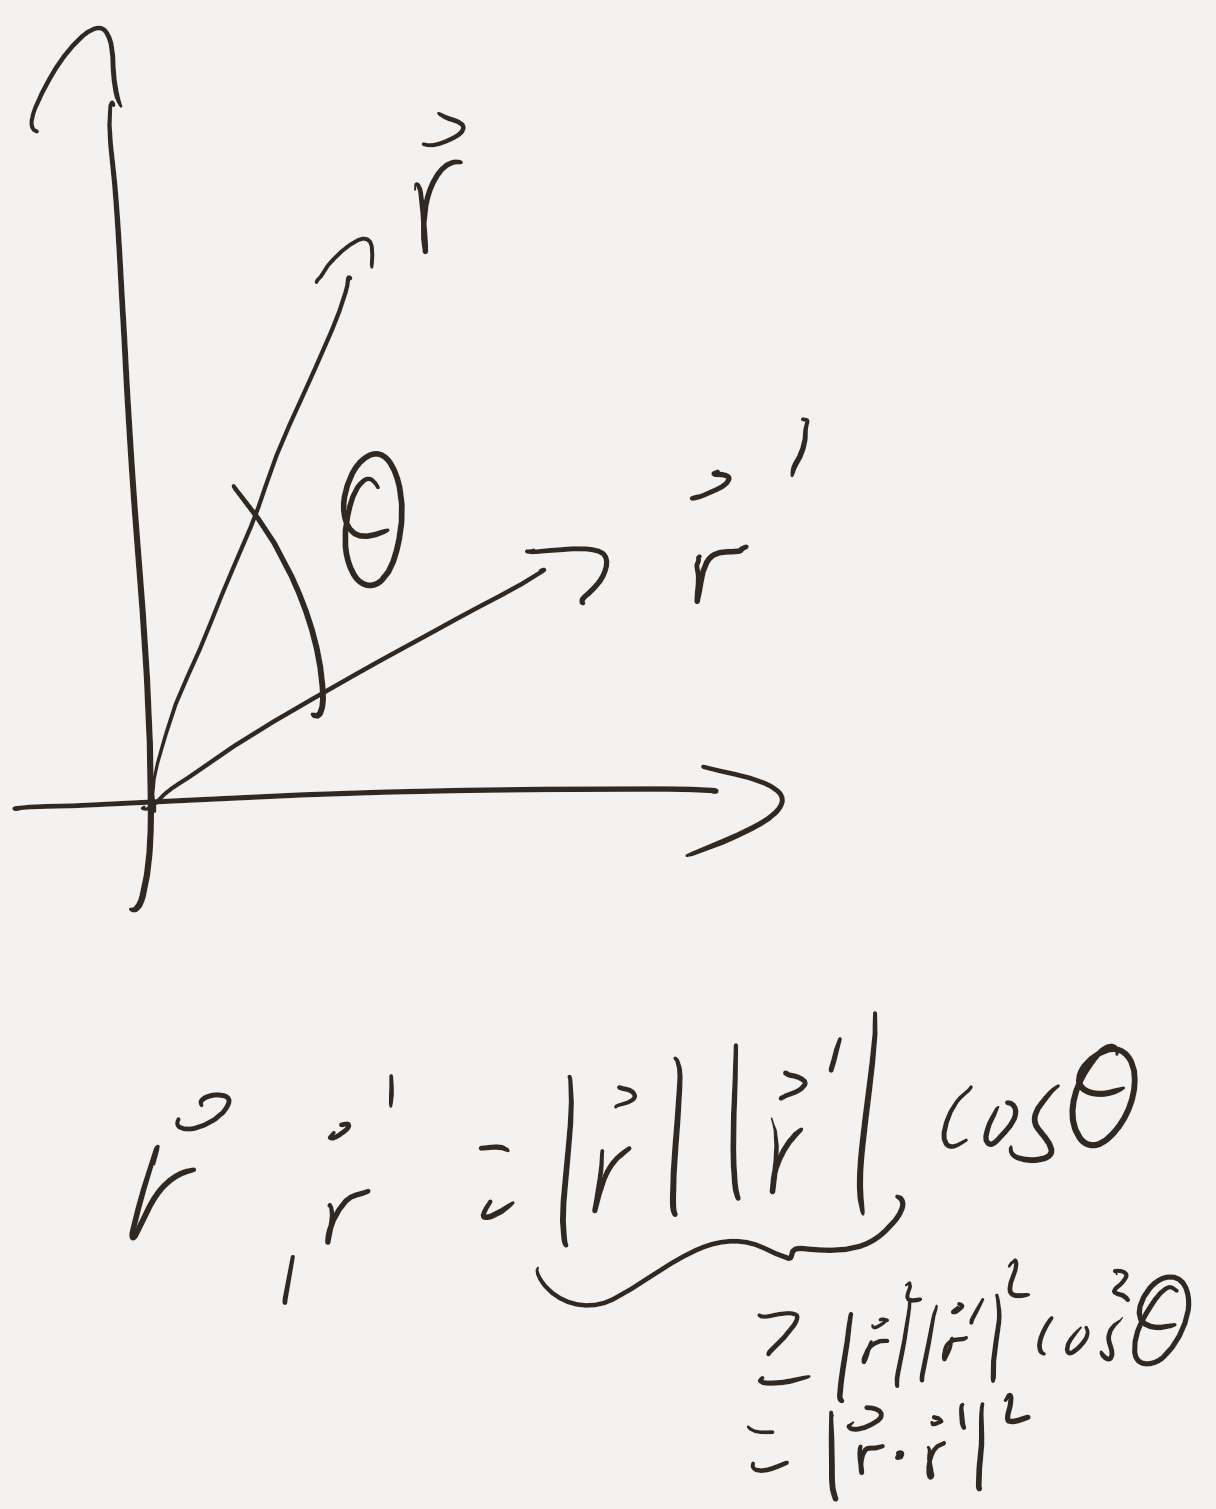
\includegraphics[width = 0.5 \textwidth]{Lecture16/1.png}

Thus, 

$$\sigma_A^2 \sigma_B^2 \geq \left( \frac{1}{2i} \langle \left[ \hat{A}, \hat{B} \right] \rangle \right)^2$$

where $[\hat{A}, \hat{B}] = \hat{A} \hat{B} - \hat{B} \hat{A}$ is referred to as the commutator of $\hat{A}$ and $\hat{B}$. 


What is the operator $[\hat{X}, \hat{p}]$? (Does it simplify?)

\begin{itemize}
    \item How would you formulate the solution to this question? i.e. what needs to be solved?
    \item How do you actually go about solving the equation?
\end{itemize}

We know how $\hat{X}$ and $\hat{p}$ work when operating on wavefunctions defined in position basis $\Longrightarrow$

$$\left( \hat{x} \hat{p} - \hat{p} \hat{x} \right) \ket{S(t)} \rightarrow \left( s \left( -i \hbar \frac{d}{dx} \right) - \left(- i \hbar \frac{d}{dx} \right) x \right) \Psi_S(x,t)$$

$[\hat{x}, \hat{p}]$: the canonical commutation relationship. As we increase degrees of freedom in our problem, there will be much more than just position and momentum. It is very natural to identify, in any particular problem, a set of canonically related variables, like position and momentum, There will be angular version of this, and in electromagnetism for example, there are even more, often more subtle, canonically related variables. 

%The more generic derivation of the example we described above:

%slide 12

%slide 13

\subsection{Exercise}

Derive the uncertainty principle prediction for the relationship between the variances of the energy and momentum operators for a free particle. 

$$\sigma_p^2 \sigma_E^2 = ?$$

It is proportional to $[\hat{p}, \hat{E}]$

$\hat{E} = \hat{H} = \frac{\hat{p}^2}{2m} \Rightarrow \text{ need } [\hat{p}, \hat{p}^2] = 0$

Keep the following in mind:

$$[\hat{A}^2, \hat{B}] = \hat{A} [\hat{A}, \hat{B}] + \hat{A}, \hat{B}] \hat{A}$$

$$[\hat{A}, \hat{B}^2] = \hat{B} \hat{A}, \hat{B}] + [\hat{A}, \hat{B}] \hat{B}$$

$$[\hat{p}, \hat{p}^2] = \hat{p} \underbrace{[\hat{p}, \hat{p}]}_{ = 0} + \underbrace{[\hat{p}, \hat{p}]}_{= 0} \hat{p}$$

The fact that $\sigma_p^2 \sigma_E^2 \geq 0$ means $\sigma_p^2 \sigma_E^2$ can be $=0$

\subsection{Exercise}

Derive the uncertainty principle prediction for the relationship between the variances of the energy and momentum operators for a particle in a harmonic oscillator potential. 

$$\hat{E} = \hat{H} = \frac{\hat{p}^2}{2m} + \frac{k}{2} \hat{x}^@ \Rightarrow [\hat{p}, \hat{H}] = \underbrace{[\hat{p}, \frac{\hat{p}}{2m}]}_{=0} + [\hat{p}, \frac{k}{2} \hat{x}^2]$$

$$\frac{k}{2} [\hat{p}, \hat{x}^2] = \frac{k}{2} \left( \hat{x} \underbrace{[\hat{p}, \hat{x}]}_{=-i \hbar} + \underbrace{[\hat{p}, \hat{x}]}_{=-i \hbar} \hat{x} \right)$$

$$\Rightarrow \sigma_p^2 \sigma_E^2 |_{HO} \geq \frac{\hbar^2 k^2}{4} \langle \hat{x} \rangle^2$$


\subsection{Last: Observations}


What sense can you make of 

\begin{enumerate}
    \item the differences between these two results, and
    \item the fact that the parameter that characterizes the minimum value of the product of uncertainties in one case depends on $\langle x \rangle$?
\end{enumerate}




\end{document}